\begin{description}
\itemsep1pt\parskip0pt\parsep0pt
\item[Keywords]
statistics, smoothing, error analysis
\end{description}

\pagebreak

\section{Overview}\label{OV}

This package is an implementation of a local polynomial kernel estimator
(LPKE) along with utilities for smoothing a CDI file and performing an
eigen-variation analysis. The package contains a generic implementation
of an LPKE that can be customized to any polynomial order, domain
dimensionality, numeric type, kernel function, and coordinate scaling.
It also provides a convenience class for loading 1D, 2D, and 3D ROOT
data from a \texttt{TH1} or \texttt{TGraphErrors}.\\The utilities for
smoothing a CDI file and performing the eigen-variation (EV) analysis
are meant to aid in production of the smoothed CDI calibrations file and
perform a complete EV analysis to help decide the appropriate number of
EV to keep, respectively. They should be run from the command line as
standalone executables and are not ROOT macros.\\These utilities allow
for some customizability, but in general will require modifications to
their respective source codes for more realistic scenarios. The utility
for smoothing a CDI file allows for command-line specification of the
file to smooth, the number of $p_T$ bins to store, and the (global)
bandwidth. To specify which data sets to smooth, order of LPKE, etc. one
needs to look at \texttt{smoothCalibrations.cxx}. The utility for the EV
analysis can be customized at the command line to specify the required
files, number of desired EV, and which data set to look analyze.

\section{Quick Start}\label{quick-start}

Here are the steps to quickly get up and running with smoothing a CDI
file and run the eigen-variation analysis on LXPLUS (warning - some
directories may need to change, but code works):

\begin{itemize}
\itemsep1pt\parskip0pt\parsep0pt
\item
  Setup proper ROOT version (needs C++11)

  \begin{enumerate}
  \def\labelenumi{\arabic{enumi}.}
  \itemsep1pt\parskip0pt\parsep0pt
  \item
    \texttt{localSetupROOT 6.02.10-x86\_64-slc6-gcc48-opt}
  \end{enumerate}
\item
  Checkout and setup RootCore

  \begin{enumerate}
  \def\labelenumi{\arabic{enumi}.}
  \item
\begin{verbatim}
svn co svn+ssh://svn.cern.ch/reps/atlasoff/PhysicsAnalysis/
D3PDTools/RootCore/tags/`svn ls svn+ssh://svn.cern.ch/reps/
atlasoff/PhysicsAnalysis/D3PDTools/RootCore/tags | 
tail -n 1` RootCore
\end{verbatim}
  \item
    \texttt{source RootCore/scripts/setup.sh}
  \end{enumerate}
\item
  Checkout relevant packages

  \begin{enumerate}
  \item
\begin{verbatim}
rc checkout_pkg atlasoff/PhysicsAnalysis/JetTagging/
JetTagPerformanceCalibration/CalibrationDataInterface/trunk
\end{verbatim}
  \item
\begin{verbatim}
rc checkout_pkg atlasoff/PhysicsAnalysis/JetTagging/
JetTagPerformanceCalibration/CDIFiles/trunk
\end{verbatim}
  \item
\begin{verbatim}
rc checkout_pkg atlasperf/CombPerf/FlavorTag/
JetTagPerformanceCalibration/NPandSmoothingTools/trunk
\end{verbatim}
  \end{enumerate}
\item
  Compile packages

  \begin{enumerate}
  \itemsep1pt\parskip0pt\parsep0pt
  \item
    \texttt{rc find\_packages}
  \item
    \texttt{rc compile}
  \end{enumerate}
\item
  Run smoothing procedure

  \begin{enumerate}
  \itemsep1pt\parskip0pt\parsep0pt
  \item
    \texttt{ln -s NPandSmoothingTools/scripts/RUN\_SMOOTHING.sh .}
  \item
    \texttt{source RUN\_SMOOTHING.sh}
  \end{enumerate}
\item
  Run EV analysis

  \begin{enumerate}
  \item
\begin{verbatim}
ln -s NPandSmoothingTools/scripts/RUN_EIGEN_ANALYSIS.sh .
\end{verbatim}
  \item
    \texttt{source RUN\_EIGEN\_ANALYSIS.sh}
  \end{enumerate}
\end{itemize}

\section{Mathematical Detail}\label{mathematical-detail}

Among the most common and crucial tasks in an analysis is fitting a
curve with some functional form to a set of data. These curves are often
used to interpolate or extrapolate into critical regions of phase space.
Thus, the fitted functional form is of great importance. The form is
usually chosen with a combination of domain specific knowledge (physical
insight, etc.) and identifying those forms with previous empirical
success. However, sometimes the covariates and responses follow no
obvious or previously encountered relationship. Additionally, one might
not wish to impose a functional form on the data. In either case a
``non-parametric'' approach to constructing a smooth curve from data is
attractive.\\Broadly speaking, non-parametric curves have no innate
functional form and can in principle adapt to any set of data. Splines,
kernel estimation, and support vector regression are all forms of
non-parametric regression. Each method will model the data differently
and have its own unique ``parameters'' to determine the amount of
``smoothness'' of the curve. These are not parameters in the usual sense
of fitting because one can normally find a value of the parameter(s)
that can interpolate through all of the data. This is undesirable in our
context (otherwise, one could just use a histogram or empirical
distribution function). There are a number of methods for constraining
the ``smoothing'' parameters, some of which are: cross validation
(REF\_HERE), minimization of squared residuals (REF\_HERE), or aesthetic
(REF\_HERE).

\subsection{Local Polynomial Kernel
Estimator}\label{local-polynomial-kernel-estimator}

The method described here is called local polynomial kernel estimation.
One can think of this method as fitting a polynomial by weighted least
squares where the weights are functions of the covariates. These
``weight'' functions are referred to as kernels. A general, multivariate
local polynomial kernel estimator of polynomial order $p$, covariate
dimension $d$, with kernel $K(\mathbf{x})$, $d\times d$ bandwidth matrix
$\mathbf{H}$, and constructed from $n$ data points with covariates
$\mathbf{X}_{i}$ and responses $Y_i$ has the form: \[
\hat{m}(\mathbf{x};p,\mathbf{H})=\hat{\mathbf{e}}^T_1\cdot\left(
\mathbf{X}^T_{\mathbf{x}}\mathbf{W}_{\mathbf{x}}
\mathbf{X}_{\mathbf{x}}\right)^{-1}\mathbf{X}^T_{\mathbf{x}}
\mathbf{W}_{\mathbf{x}}\mathbf{Y}
\] where, \[
\mathbf{W}_{\mathbf{x}}=
\begin{bmatrix}
K_{\mathbf{H}}(\mathbf{X}_1-\mathbf{x}) &  \ldots & 0\\
\vdots  &  \ddots & \vdots\\
0  &\ldots & K_{\mathbf{H}}(\mathbf{X}_n-\mathbf{x})
\end{bmatrix}
\] \[
\mathbf{Y}=
\begin{bmatrix}
Y_1 \\
\vdots \\
Y_n
\end{bmatrix}
\] \[
\mathbf{X}_{\mathbf{x}}=
\begin{bmatrix}
1 & \left(\overrightarrow{\Delta}^1_1\right)^T &  \ldots & \left(\overrightarrow{\Delta}^p_1\right)^T\\
\vdots & \vdots &  \ddots & \vdots\\
1 & \left(\overrightarrow{\Delta}^1_n\right)^T &  \ldots & \left(\overrightarrow{\Delta}^p_n\right)^T\\
\end{bmatrix}
\]

\[
K_{\mathbf{H}}(\mathbf{x})=\left|\mathbf{H}\right|^{-1/2}
K(\mathbf{H}^{-1/2}\mathbf{x})
\] \[
\overrightarrow{\Delta}^m_i=\sum^d_{j=1}
\left(\left(\mathbf{X}_i-\mathbf{x}\right)\cdot\hat{\mathbf{e}}_j\right)^m
\hat{\mathbf{e}}_j
\] The derivation of this for the univariate case is straightforward in
the context of least squares minimization and can be found in REF\_HERE.
In areas of phase space sufficiently far away from any data points, the
weight matrix $\mathbf{W}_{\mathbf{x}}$ will approach machine zero due
to small kernel values. The convention followed here is that in the case
of a zero weight matrix the kernel evaluations are just replaced by
\texttt{1}.\\We also allow for unequally weighted data by further
weighting the kernel by a user supplied weight, $w_i$ (default is
\texttt{1}). One should choose $w_i=1/\sigma_i^2$ if $\sigma_i$ is the
variance (for uncorrelated errors) in the responses to approximate the
best linear unbiased estimator (BLUE) (REF\_HERE). Thus, the weight
matrix looks like: \[
\mathbf{W}_{\mathbf{x}}=
\begin{bmatrix}
w_1 K_{\mathbf{H}}(\mathbf{X}_1-\mathbf{x}) &  \ldots & 0\\
\vdots  &  \ddots & \vdots\\
0  &\ldots & w_n K_{\mathbf{H}}(\mathbf{X}_n-\mathbf{x})
\end{bmatrix}
\] Lastly, for this implementation of the LPKE we use a simplified
bandwidth matrix: \[
\mathbf{H}=
\begin{bmatrix}
h_1 &  \ldots & 0\\
\vdots  &  \ddots & \vdots\\
0  &\ldots & h_d
\end{bmatrix}
\] Thus, the kernel here is a function of the ``scaled'' covariates: \[
K(\mathbf{H}^{-1/2}\mathbf{x})\rightarrow
K\left(\frac{x_1}{h_1},\ldots,\frac{x_d}{h_d}\right)
\] The $p=1$ case of the estimator is called a local linear kernel
estimator and has less bias at the ends of the data than a local
constant kernel estimator ($p=0$). Note that all odd orders have less
bias at the end points than even powers (REF\_HERE). The $p=1$ local
kernel estimator was chosen for this reason in addition to better
accommodating the spacing in the SF distributions. Below is an example
of a 6-bin scale factor distribution smoothed to 100 bins with the
kernel bandwidth of 0.6 (logarithmic
scale).\\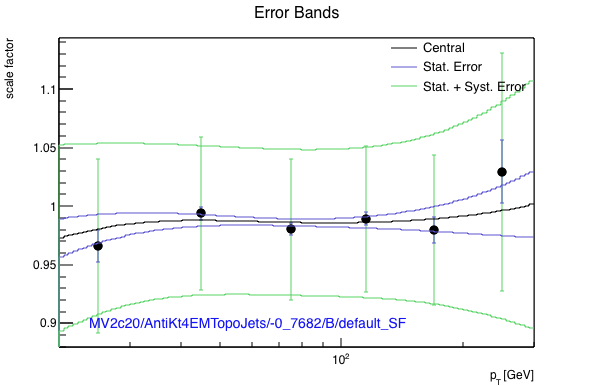
\includegraphics{media/smoothed_SF.png} Lastly, note that the
form of the estimator has the following, seemingly insignificant,
property. Let $\hat{m}_{\mathbf{Y}}$ be associated with $\mathbf{Y}$.
Now shift the $\mathbf{Y}$ by $\overrightarrow{\delta}$ so that
$\hat{m}_{\mathbf{Y}+\overrightarrow{\delta}}$ is the estimator
associated with the ``shifted'' responses. Notice that
$\hat{m}_{\mathbf{Y}+\overrightarrow{\delta}}-\hat{m}_{\mathbf{Y}}= \hat{m}_{\overrightarrow{\delta}}$.
That is to say, the estimator of the ``shifted'' responses less the
estimator for the original responses is simply the estimator associated
with the shifts themselves, $\hat{m}_{\overrightarrow{\delta}}$. This is
useful in nuisance variations where the nominal distribution is shifted
and normally one would need to perform two LPKEs and a subtraction. This
can introduce undesirable numerical effects. Fortunately, one can skip
that procedure altogether and simply perform an LPKE on the
$\overrightarrow{\delta}$'s themselves.

\subsection{Eigen-Variation Reduction}\label{eigen-variation-reduction}

Each scale factor distribution in a CDI data set has many
(\textasciitilde{}40) systematic variations as well as statistical
variations that need to be taken into account in order to properly
access the uncertainty of the distribution. For a physics analysis this
can lead to a large number of nuisance parameter when one needs to
assess the effects of various systematics. Therefore, it is highly
desirable to somehow reduce the number of systematics under
consideration.\\One method of reducing the number systematics that
preserves the bin-to-bin correlations and total error is to perform an
eigenvalue decomposition on the covariance matrix of systematic and
statistical variations, also known as a principal component analysis. It
is clear that the resulting number of variations will simply be the
number of bins in the scale factor distribution. This is already a huge
reduction of systematics to consider if your distribution has 10 bins.
However, after smoothing the number of bins can far exceed the original
number of systematics. Initially, this may seem counterproductive and
another method should be pursued. Fortunately, most of the EV are very
small in magnitude and can be thrown out without fear of losing
correlations or total error. In principle one should recover the
original number of ``significant'' EV after this pruning. The remaining
EV can be further reduced by summing up the $M$ least significant EV
(ranked by eigenvalue). Whatever summing technique is used, the over
goal is to try to satisfy the following constraint on the newly summed
histogram, $H'$: \[
H'(x_i)H'(x_j)=\sum_{k=M}^{N_{EV}}H_k(x_i)H_k(x_j)
\] This condition may only be satisfied if one of two criteria are met:

\begin{enumerate}
\def\labelenumi{\arabic{enumi}.}
\itemsep1pt\parskip0pt\parsep0pt
\item
  The $H'(x_i)$ are vectors with elements $H_k(x_i)$
\item
  The $H'(x_i)$ are scalars but the $H_k(x_i)$ conspire in such a way
  that makes this equality hold
\end{enumerate}

Unfortunately, neither of these criteria are applicable for our case.
Thus, our essential problem is that of how one can store the information
of a vector in a single scalar. Using the (false) equality above one can
set $i=j$ and take the positive square root to yield: \[
H'(x_i)=\sqrt{\sum_{k=M}^{N_{EV}}H_k^2(x_i)}
\] Using this equation ($S_Q$) preserves the total errors in the
resulting covariance matrix. However, because all the information about
the sign of the original systematics is lost this method of merging
severely distorts the correlations. Another manipulation of the (false)
equality is to first sum over $j$, sum over $i$, then finally back
substitute to solve for $H'(x_i)$: \[
H'(x_i)S_{H'}=\sum_j^{N_{\mathrm{bins}}}\sum_{k=M}^{N_{\mathrm{EV}}} H_k(x_i)H_k(x_j)
\] \[
S_{H'}^2=\sum_i^{N_{\mathrm{bins}}}\sum_j^{N_{\mathrm{bins}}}\sum_{k=M}^{N_{\mathrm{EV}}} H_k(x_i)H_k(x_j)
\] Thus, \[
\displaystyle H'(x_i)=\frac{\sum_j^{N_{\mathrm{bins}}}\sum_{k=M}^{N_{\mathrm{EV}}} H_k(x_i)H_k(x_j)}
{\sqrt{\sum_n^{N_{\mathrm{bins}}}\sum_m^{N_{\mathrm{bins}}}\sum_{k=M}^{N_{\mathrm{EV}}} H_k(x_n)H_k(x_m)}}
\] In principle this should be equal to the first method of merging,
$S_Q$. But, because the original equation is false they give different
results. This alternative method of summing ($S_A$) the $M$ lowest
eigen-variations is found empirically to better preserve the
correlations over the $S_Q$ method. However, $S_A$ doesn't preserve the
total error as $S_Q$ does. Thus, a trade off must be made as to how much
total error can be sacrificed for extra gains in correlations.\\As a
final note on EV reduction, another way of attempting to satisfy the
(false) equality is to perform a multidimensional minimization against
some metric treating each bin of the merged histogram ($H'$) as the
variables to minimize. An implementation of this using the Amoeba
routine was explored, but yielded results similar to using $S_A$. Thus,
it is not currently being used.

\section{Implementation}\label{implementation}

\subsection{LPKE}\label{lpke}

The LPKE implemented in this package (\texttt{LocalPolyKernelEstimator})
attempts to be as generic as possible. It is written in idiomatic C++11
and requires a compatible ROOT version (version 6 or version 5 with the
c++11 flag enabled). The \texttt{LocalPolyKernelEstimator} class allows
for any domain dimension, order of estimator, coordinate scaling, or
kernel function (albeit the kernel must be a function of an array of
normalized coordinates). It is a straightforward and naive
implementation with respect to computational efficiency and numerical
stability. No effort is made to reduce the number of kernel evaluations
with a nearest-neighbors-based pruning or ensure that the minimum number
of numerically unstable operations are performed. However, for our
applications this doesn't appear to be an issue.\\The coordinate scaling
and kernel types are fed into the template parameters for
\texttt{LocalPolyKernelEstimator}. The coordinate scaling function must
take a single parameter (unnormalized coordinate) that returns the
scaled coordinate. The kernel function should accept an
\texttt{std::array} that represents the set of normalized coordinates
and should return the value of the kernel at that coordinate.\\The
convenience class \texttt{LocalLinearKernelEstimator1D} is provided to
easy the smoothing of a ROOT \texttt{TH1} or \texttt{TGraphErrors}. In
addition to requiring a coordinate transform function an inverse
coordinate transform is necessary to properly construct the smoothed
histogram. It allows the easy retrieval of a smoothed \texttt{TH1D}
given the number of bins to smooth to.\\The utility for smoothing a
given CDI file is \texttt{smoothCalibrations}. This is relatively simple
routine that gathers the CDI datasets from a CDI file, smooths the
relevant histograms, writes the ``ReducedSets'' numbers, and stores them
in a new CDI file. Which datasets it smooths are hard coded as well as
the EV ``ReducedSets'' numbers. It checks each histogram to identify the
systematics with uncorrelated bins. Those with uncorrelated bins are
smoothed bin-by-bin to account for the bin-to-bin independence. Thus,
one systematic with $N$ uncorrelated bins will be stored as $N$ smoothed
systematics with correlated bins. The central value (denoted ``result''
in the dataset) is smoothed using the bin errors as weights. All other
histograms are smoothed without using bin errors. Finally, the current
implementation smooths only along $p_T$. It treats each $\eta$ bin as a
separate \texttt{TH1D} along $p_T$.

\subsection{Eigen-Variation Analysis}\label{eigen-variation-analysis}

The eigen-variation analysis utility is designed to aid in the
determination of the appropriate number of EV to merge. Running this
analysis executable yields two files:

\begin{enumerate}
\def\labelenumi{\arabic{enumi}.}
\itemsep1pt\parskip0pt\parsep0pt
\item
  A ROOT file with plots of the EV, central value, statistical nuisance
  analysis, percent difference of covariance matrices, etc.
\item
  A text file with information on the average and maximum relative
  differences for total error, correlations, etc.
\end{enumerate}

This can then be used to determine an acceptable amount of EV merging.
The number of EV before any merging should be the about the same as the
number of EV before smoothing.

\section{Usage}\label{usage}

\subsection{LPKE}\label{lpke-1}

The \texttt{LocalPolyKernelEstimator} class needs to be initialized with
several template parameters:

\begin{enumerate}
\def\labelenumi{\arabic{enumi}.}
\itemsep1pt\parskip0pt\parsep0pt
\item
  \texttt{size\_t Dim}: this is the desired domain dimension
\item
  \texttt{size\_t Order}: this is the desired order of estimator
\item
  \texttt{typename CoordTransformFunc\_t}: the type of the coordinate
  transformation function
\item
  \texttt{typename KernelFunc\_t}: the type of the kernel function
\item
  \texttt{typename Numeric\_t}: the numeric type to use in computation
\end{enumerate}

Evaluation of this class is through the `()' operator that takes either
a variable number of arguments or an array of coordinates (length
\texttt{DIM}). Setting the coordinate data is accomplished through two
functions; \texttt{SetCoordinate} and \texttt{AddCoordinate}. Both of
these function accept either a variable number of arguments or an array
of coordinates (length \texttt{DIM} + 2 or \texttt{DIM} + 1).
Specifically, they need the domain coordinates along with the response
coordinate and (optionally) the error associated with the response.
\texttt{SetCoordinate} is best used in conjunction with
\texttt{SetNumberOfCoordinates} method to reserve the exact number of
data points needed or if you know the index of the point.
\texttt{AddCoordinate} is convenient for quickly adding an additional
data point. Modifying a coordinate can be accomplished through the
\texttt{SetCoordinate} function with the appropriate index. The
bandwidth should be set along each dimension with the function
\texttt{SetBandwidth} and will be used to create the normalized
coordinates.\\The \texttt{LocalLinearKernelEstimator1D} class is a
simplification of the \texttt{LocalPolyKernelEstimator} class that eases
the creation of a smoothed \texttt{TH1D}. It has no template parameters
of it's own and is effectively \texttt{LocalPolyKernelEstimator} with
the following template parameters set:

\begin{enumerate}
\def\labelenumi{\arabic{enumi}.}
\itemsep1pt\parskip0pt\parsep0pt
\item
  \texttt{Dim = 1}
\item
  \texttt{Order = 1}
\item
  \texttt{CoordTransformFunc\_t = std::function\textless{}double(double)\textgreater{}}
\item
  \texttt{KernelFunc\_t = std::function\textless{}double(const std::array\textless{}double, 1\textgreater{}\&)\textgreater{}}
\item
  \texttt{Numeric\_t = double}
\end{enumerate}

It adds a function to set the number of bins, set the inverse coordinate
transform, load data from a \texttt{TH1} or \texttt{TGraphErrors}, and
make a smoothed \texttt{TH1D}.\\Example usage:

\hyperdef{}{mycode}{\label{mycode}}
\begin{Shaded}
\begin{Highlighting}[numbers=left,,]
    \KeywordTok{using} \NormalTok{KernelSmoother = Analysis::LocalLinearKernelEstimator1D;}
    \NormalTok{KernelSmoother smoother;}
    \NormalTok{smoother.SetNbins(}\DecValTok{100}\NormalTok{);}
    \NormalTok{smoother.SetCoordTransform(}\DecValTok{0}\NormalTok{, TF1(}\StringTok{"log scale"}\NormalTok{, }\StringTok{"log(x)"}\NormalTok{, }\DecValTok{1}\NormalTok{, }\DecValTok{10}\NormalTok{));}
    \NormalTok{smoother.SetInvCoordTransform(}\DecValTok{0}\NormalTok{, TF1(}\StringTok{"exp scale"}\NormalTok{, }\StringTok{"exp(x)"}\NormalTok{, }\DecValTok{1}\NormalTok{, }\DecValTok{10}\NormalTok{));}
    \KeywordTok{using} \NormalTok{Coord_t = }\KeywordTok{typename} \NormalTok{KernelSmoother::Coord_t<KernelSmoother::DIM>;}
    \NormalTok{TF1 k1D(}\StringTok{"kernel"}\NormalTok{, }\StringTok{"TMath::Gaus(x, 0, 1, 1)"}\NormalTok{, }\DecValTok{-1}\NormalTok{, }\DecValTok{1}\NormalTok{);}
    \KeywordTok{auto} \NormalTok{kernel = [k1D](}\DataTypeTok{const} \NormalTok{Coord_t &coord) \{}\KeywordTok{return} \NormalTok{k1D(coord[}\DecValTok{0}\NormalTok{]);\};}
    \NormalTok{smoother.SetKernel(kernel);}
    \NormalTok{smoother.SetBandwidth(}\DecValTok{0}\NormalTok{, }\FloatTok{0.}\DecValTok{4}\NormalTok{);}
    \NormalTok{smoother.UseErrorWeights(}\KeywordTok{false}\NormalTok{);}
    \CommentTok{// ...}
    \CommentTok{// import 1D histogram to_smooth}
    \CommentTok{// ...}
    \NormalTok{smoother.LoadData(to_smooth);}
    \KeywordTok{auto} \NormalTok{smoothed = smoother.MakeSmoothedTH1D();}
    \CommentTok{// ...}
\end{Highlighting}
\end{Shaded}

The utility to smooth a CDI file is the \texttt{SmoothCDI} executable.
It takes the following command line arguments:

\begin{enumerate}
\def\labelenumi{\arabic{enumi}.}
\itemsep1pt\parskip0pt\parsep0pt
\item
  the input CDI file to smooth
\item
  (optional: default = 100) the number of smooth bins
\item
  (optional: default = 0.4) the global bandwidth for the $p_T$ axis for
  the kernel smoother
\end{enumerate}

Look at \texttt{scripts/RUN\_SMOOTHING.sh} for example usage.

\subsection{Eigen-Variation Analysis}\label{eigen-variation-analysis-1}

The utility to analyze eigen-variations is the
\texttt{AnalyzeEigenVariation} executable. It takes the following
command line arguments:

\begin{enumerate}
\def\labelenumi{\arabic{enumi}.}
\itemsep1pt\parskip0pt\parsep0pt
\item
  the input smoothed CDI file
\item
  an unsmoothed CDI file used for reference
\item
  the full path to the CDI dataset to analyze
\item
  (optional: default = -1) the number of EV to merge in the smoothed EV
  set, default is none
\item
  (optional: default = true) deprecated
\end{enumerate}

Look at \texttt{scripts/RUN\_EIGEN\_ANALYSIS.sh} for example usage.
